\documentclass[a4paper,12pt]{report}
\usepackage[utf8]{inputenc}
\usepackage[T1]{fontenc}
\usepackage[english]{babel}
\usepackage{lmodern}

%hyperref for interactive PDF index
\usepackage[bookmarks, colorlinks, breaklinks]{hyperref}
\hypersetup{linkcolor=black, citecolor=black, filecolor=black, urlcolor=black}

%Package required to use figures
\usepackage{graphicx}
%Include the bibliography in the table of contents
\usepackage{tocbibind}

%Our chapters must be called sections
\addto\captionsenglish{\renewcommand{\chaptername}{Section}}

\begin{document}

%Code for title page
\begin{titlepage}
\centering
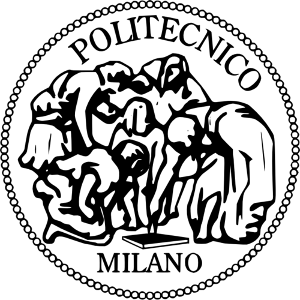
\includegraphics[width=0.20\textwidth]{./pictures/logo_poli}\par
	\vspace{1.5cm}
	{\Large {PowerEnJoy \\ 
		Software Engineering II} \par}
	\vspace{1.5cm}
	{\LARGE \textbf{Requirements Analysis and Specification Document} \par}
	\vspace{1.5cm}
	{\Large\itshape Giovanni Scotti, Marco Trabucchi\par}
	\vspace{2cm}
	\vfill
	% Bottom of the page
	{\large \today \par}
\end{titlepage}

%Make the table of contents
\tableofcontents

%INTRODUCTION
\chapter{Introduction}
\label{ch:Introduction}

\section{Purpose}
%purpose
The Design Document is intended to provide a deeper functional description of the \emph{PowerEnJoy} system-to-be by giving technical details and describing the main architectural components as well as their interfaces and their interactions. The relations among the different modules are pointed out using UML standards and other useful diagrams showing the structure of the system.

The document aims to guide the software development team to implement the architecture of the project, by providing a stable reference and a single vision of all parts of the software itself and clearly defining how they work.

\section{Scope}
The product is a digital management system to support a car-sharing service that exclusively employs electric cars.

The system consists of a back-end server application that manages rental requests remotely and three front-end applications:

\begin{itemize}
\item A web-based application to provide the final user with a friendly interface to take advantage of the services of \hbox{\emph{PowerEnJoy}};
\item An application that runs on the existing on-board computers provided on each vehicle, used to interact with the car itself, unlock it and access the GPS/sat-nav service;
\item A mobile application that allows the user to easily access the service anywhere he/she needs to.
\end{itemize}
%serve per modellare i requisiti relativi al sw del computer di bordo [vd specifiche p.3 sez.5]
%"The user is notified of the current charges through a screen on the car"

The system is intended for only one type of user: drivers, who should be allowed to register and access the system via username and password, in order to make the renting and payment processes easier and quicker to carry out. Moreover, the system aids the users by locating nearby available vehicles and keeps track of the distance driven, all while notifying them about the amount of money they are being charged. Predefined safe parking areas are signaled by an on-board computer.

Lastly, the system aims to motivate drivers to maintain a virtuous behavior providing discounts when it detects signs of responsible and ecologic actions.


\section{Definitions, Acronyms and Abbreviations}
\begin{description}
\item[RASD:] Requirements Analysis and Specification Document.
\item[System:] The software system-to-be, in all of its entirety.
\item[Driver:] See \textbf{User}.
\item[User:] Any person subscribed to the service who rents a car using \hbox{\emph{PowerEnJoy}}.
\end{description}



\section{References}
This document follows the guidelines provided by ISO/IEC/IEEE 29148:2011~\cite{ieee-29148} and IEEE 830-1998~\cite{ieee-830} respectively related to the requirements engineering for systems and software products and the recommended practice for software requirements specifications.

Moreover it is strictly based on the specifications concerning the RASD assignment~\cite{se-assignments} for the Software Engineering II project, part of the course held by professors Luca Mottola and Elisabetta Di Nitto at the Politecnico di Milano, A.Y. 2016/17.

\section{Overview}
This document consists of three sections:

\begin{description}
\item[Section 1: Introduction.] A general introduction and overview of the system-to-be purpose, scope and goals, along with some important information about this document.
\item[Section 2: Overall description.] It describes the general factors that affects the product and its requirements. The section provides a background for those requirements which are defined in detail in Section 3 and makes them easier to figure out.
\item[Section 3: Specific Requirements.] All the software requirements are specified to a level of detail which is sufficient to let the designers satisfy them. Both functional and non-functional requirements are mentioned.
\end{description}
At the end of the document are an \textbf{Appendix} and a \textbf{Bibliography}, providing additional information about the sections listed above.

\chapter{Overall Description}
\label{ch:Overall Description}

\section{Product Perspective}
%This should list each system interface and identify the functionality of the software to accomplish the system requirement and the interface description to match the system.
\subsection{User interfaces}
The users have two ways to access the system: a web application can be executed on any personal computer while a mobile application provides flexibility, portability and can be used literally everywhere. Despite the fact that the hardware interfaces running the application are rather different, a unified and common user interface is provided. It should be user friendly and very intuitive to allow everyone to easily use it without any specific knowledge.

Moreover the users have to interact with the on-board computer installed on each electric vehicle, therefore it should offer an interface as straightforward as the one implemented by the web and mobile applications.

%INSERIRE IL REFERENCE A CONSTRAINTS
\subsection{Hardware interfaces}
The web application can be executed on any general purpose computer that complies with the minimum system requirements specified in subsection \ref{ssec:hlimit}.

The mobile application has to exchange data with the GPS module located on any recent smart-phone. Moreover it has to access the mobile broadband in order to communicate with the main system server.

An on-board computer is set up in each electric car and it talks to the vehicle control unit through the CAN bus and to the system server via the mobile broadband.

\subsection{Software interfaces}
The web based application must support the main browsers such as IE, Google Chrome and Mozilla Firefox. The mobile application has to be compatible with iOS and Android. The server side of the application, that is the system back-end, stores data in a relational DBMS and runs on any web server that supports Java.
%DA RIVEDERE
The back-end has mainly to deal with:
\begin{itemize}
\item car reservation
\item payments
\item data storage and management
\item customer account maintenance
\end{itemize}

\section{Product Functions}
The system allows users to reserve available cars, to manage their requests and charge them for the rental.

The users can:
\begin{itemize}
\item Register to the service;
\item Login with their personal account;
\item Edit and manage personal information;
\item Delete their existing account;
\item Locate nearby available-to-rent vehicles;
\item Reserve one of said cars for a fixed amount of time;
\item Unlock the reserved vehicle based on their mobile device GPS position;
\item Alternatively, unlock the reserved car by inserting a vehicle-specific code (found on the windshield) into the application;
\item Start the engine by inserting their PIN;
%solo cose che può fare o anche informazioni che può ricevere? notifica parcheggi e spesa corrente
\item Perform payments for the used service via credit card or \emph{PayPal\textsuperscript{TM}}.
\end{itemize}

\section{User Characteristics}
Target of the service are \emph{drivers} that wish to rent a car.

The base assumption is that every registered user is in possess of a driving license which is valid in the country where he/she makes use of the service.

Moreover, the user must have the means of accessing the service from anywhere: this includes having the possibility to use a stable internet connection both from a mobile device and a stationary one such as a laptop or desktop PC.

Lastly, the user should provide the system a valid payment method upon the act of registration to the service.

\section{Constraints}
\subsection{Regulatory policies}
The system must be allowed by the user to collect, process and store personal data. Furthermore the system is capable to delete all the personal data on user request and to keep track of each payment.

The user has the responsibility to use the system properly in order to comply with the local laws and policies.

\subsection{Hardware limitations}
The system should met the following limitations:
\begin{itemize}
\item Mobile application:
	\begin{itemize}
	\item[>] 3G UMTS connection at its maximum speed of 2 Mb/s
	\item[>] 50 MB of available space
	\item[>] 1 GB of RAM
	\item[>] GPS module
	\end{itemize}
\item Web application:
	\begin{itemize}
	\item[>] Internet connection at 7 Mb/s
	\item[>] 800x600 screen resolution
	\end{itemize}
\end{itemize}

\subsection{Parallel operation}
The system must support parallel operations from different users and the DBMS relies heavily on concurrent transactions.

\subsection{Reliability requirements}
The system reliability, that is the probability to operate without a failure for a specific period of time, must be 99\%.

\subsection{Criticality of the application}
Life-critical applications do not concern the system to be developed.

\appendix
\chapter{Appendix}
\section{Software and tools used}
\begin{itemize}
\item \LaTeX, used as typesetting system to build this document.
\item draw.io - \url{https://www.draw.io} - used to draw diagrams and mock-ups.
\item GitHub - \url{https://github.com} - used to manage the different versions of the document and to make the distributed work much easier.
\item GitHub Desktop, the GitHub official application that offers a seamless way to contribute to projects.
\end{itemize}
\section{Hours of work}
The absolute major part of the document was produced in group work. The approximate number of hours of work for each member of the group is the following:

\begin{itemize}
\item Giovanni Scotti: 25 hours
\item Marco Trabucchi: 20 hours
\end{itemize}

NOTE: indicated hours include the time spent in group work.

\begin{thebibliography}{1}

\bibitem{ieee-29148}
	ISO/IEC/IEEE 29148:2011 \emph{Systems and software engineering - Life cycle processes - Requirements engineering}
	
\bibitem{se-assignments}
	AA 2016/2017 Software Engineering 2 - \emph{Project goal, schedule and rules}

\end{thebibliography}

\end{document}